\subsection{Netrek}\label{subsec:netrek}

The last game we will discuss is \textit{Netrek} (1989).\ \textit{Netrek} began as \textit{Xtrek}, a game inspired by \textit{Empire} (1973), a strategy game for the PLATO system loosely based on the Star Trek universe~\cite{netrekhist}.\ \textit{Xtrek} used the X Window System for UNIX on a client-server architecture, though the remote server was responsible for driving the display as well as handling server-side game logic.\ \textit{Netrek} was built from this, replacing the server-driven display with client-side rendering, leaving the server as the controller of the world state. Both games used TCP/IP to communicate, and ran on any UNIX device with an internet connection and X10 support. In 1989, the source code for \textit{Netrek} was uploaded to Usenet, and subequent iterations have remained open source ever since.

Players of \textit{Netrek} control spaceships in a large shared galaxy within which the objective is to capture as many planets for your chosen team as possible. Maximum players could be specified by the server owner, though the default value is 20. All interactions happen in real time, and the game considers itself more of a sport than a video game, necessitating features which maintain competitive integrity (\eg{} cheat-mitigation, low latency, and minimal transmission error).

Historical source code, written in C, is available on Netrek.org's ftp archive~\cite{netreksrc}. The oldest version we could find was last updated in 1992. Features added after our 1989 cutoff (UDP transmission and RSA encryption) are modularly used, so we can easily ignore them in our static analysis. By doing so, we are looking at code that is as similar as possible to the original 1989 Usenet submission.

\textit{Netrek} was designed to be flexible. Servers were intended to easy to set up and were highly configurable through config files. Server administrators could modify rules of the game on the fly, and the server would periodically read the config files and update the game without requiring a restart or any interruption to the game. Since hosting was not centralized, players needed a directory to find active games. Metaservers were created, which simply hosted a static list of \textit{Netrek} servers that could be updated by the metaserver owner and checked if they were running. We were unable to find any evidence of metaservers in video games predating \textit{Netrek}, so it may be the first to use this.

Servers would also maintain records of users and their statistics in the game. Upon connecting to a server, the main thread of the server would create a thread to handle all communication to that player. Then, the user would enter a username and password to register or log in. Passwords were hashed with the standard POSIX \mono{crypt} library, using the DES algorithm with the username as salt. If the server was full (maximum number of players already connected), connecting players could be placed into a queue, from which new players would join when another player disconnected.

Similar to \textit{Habitat}, the server places no trust in the information sent by the client. In complete opposition to \textit{Maze} where clients inform the server of state changes, \textit{Netrek} clients send requests to the server, which will update the world state if the request is valid. For instance, a player cannot set their ship's speed above its maximum, as this request would simply be ignored. The player thread on the server handles this logic, and if a request is accepted, the relevant state change is written to memory which is shared by all player threads and the main thread. This state is limited to simple information like ship speed and direction, and only the player thread writes to this area of memory. No mutexes, locks, or any other measures are used to mitigate race conditions; only the design of the software prevents them.

To update the world state with more complex data such as player position, player fuel, projectile weapon position and hit detection, or planet status, the main thread periodically reads from the shared memory and performs calculations to update this information. Therefore the main daemon handles no networking except to fork a player thread and pass it the socket used to communicate with the player. World state is periodically sent to the player at a user-configurable rate, the most common being 5 updates per second.

This architecture meant that the server had full control over the world state, and clients simply block until the user sends an inputs or until it is time to receive the new world state.

Connectivity would have been more robust than the earlier games we reviewed, as the game supported seamless reconnection if the client disconnected without requiring a new log in or losing the client's state. The use of TCP packets would have also guaranteed error-free and in-order transmission. Unlike in Quantum Link, the developers did not need to write any of this logic themselves as it was handled by the kernel-level implementation.

Since TCP packets were used, we will not go into the details of the overall packet structure as this is well documented. Of more interest is the structure of the packet's payload. Payloads are fairly simple, consisting of a single byte for \mono{type}, with following bytes being additional information. Once again proving different to earlier networked games, \textit{Netrek} has many different types of payloads instead of having a generic \mono{DATA} payload that others have. There are 26 server payload types, and 33 client payload types. Each is specific to one purpose, \eg{} \mono{CP\_SPEED} is a request by the client to change their speed, and \mono{SP\_PLAYER} updates the player on their new location. We will not list all 59 payload types here, but instead show a few examples of them in the following diagrams.

% Registration
\begin{figure}[h]
  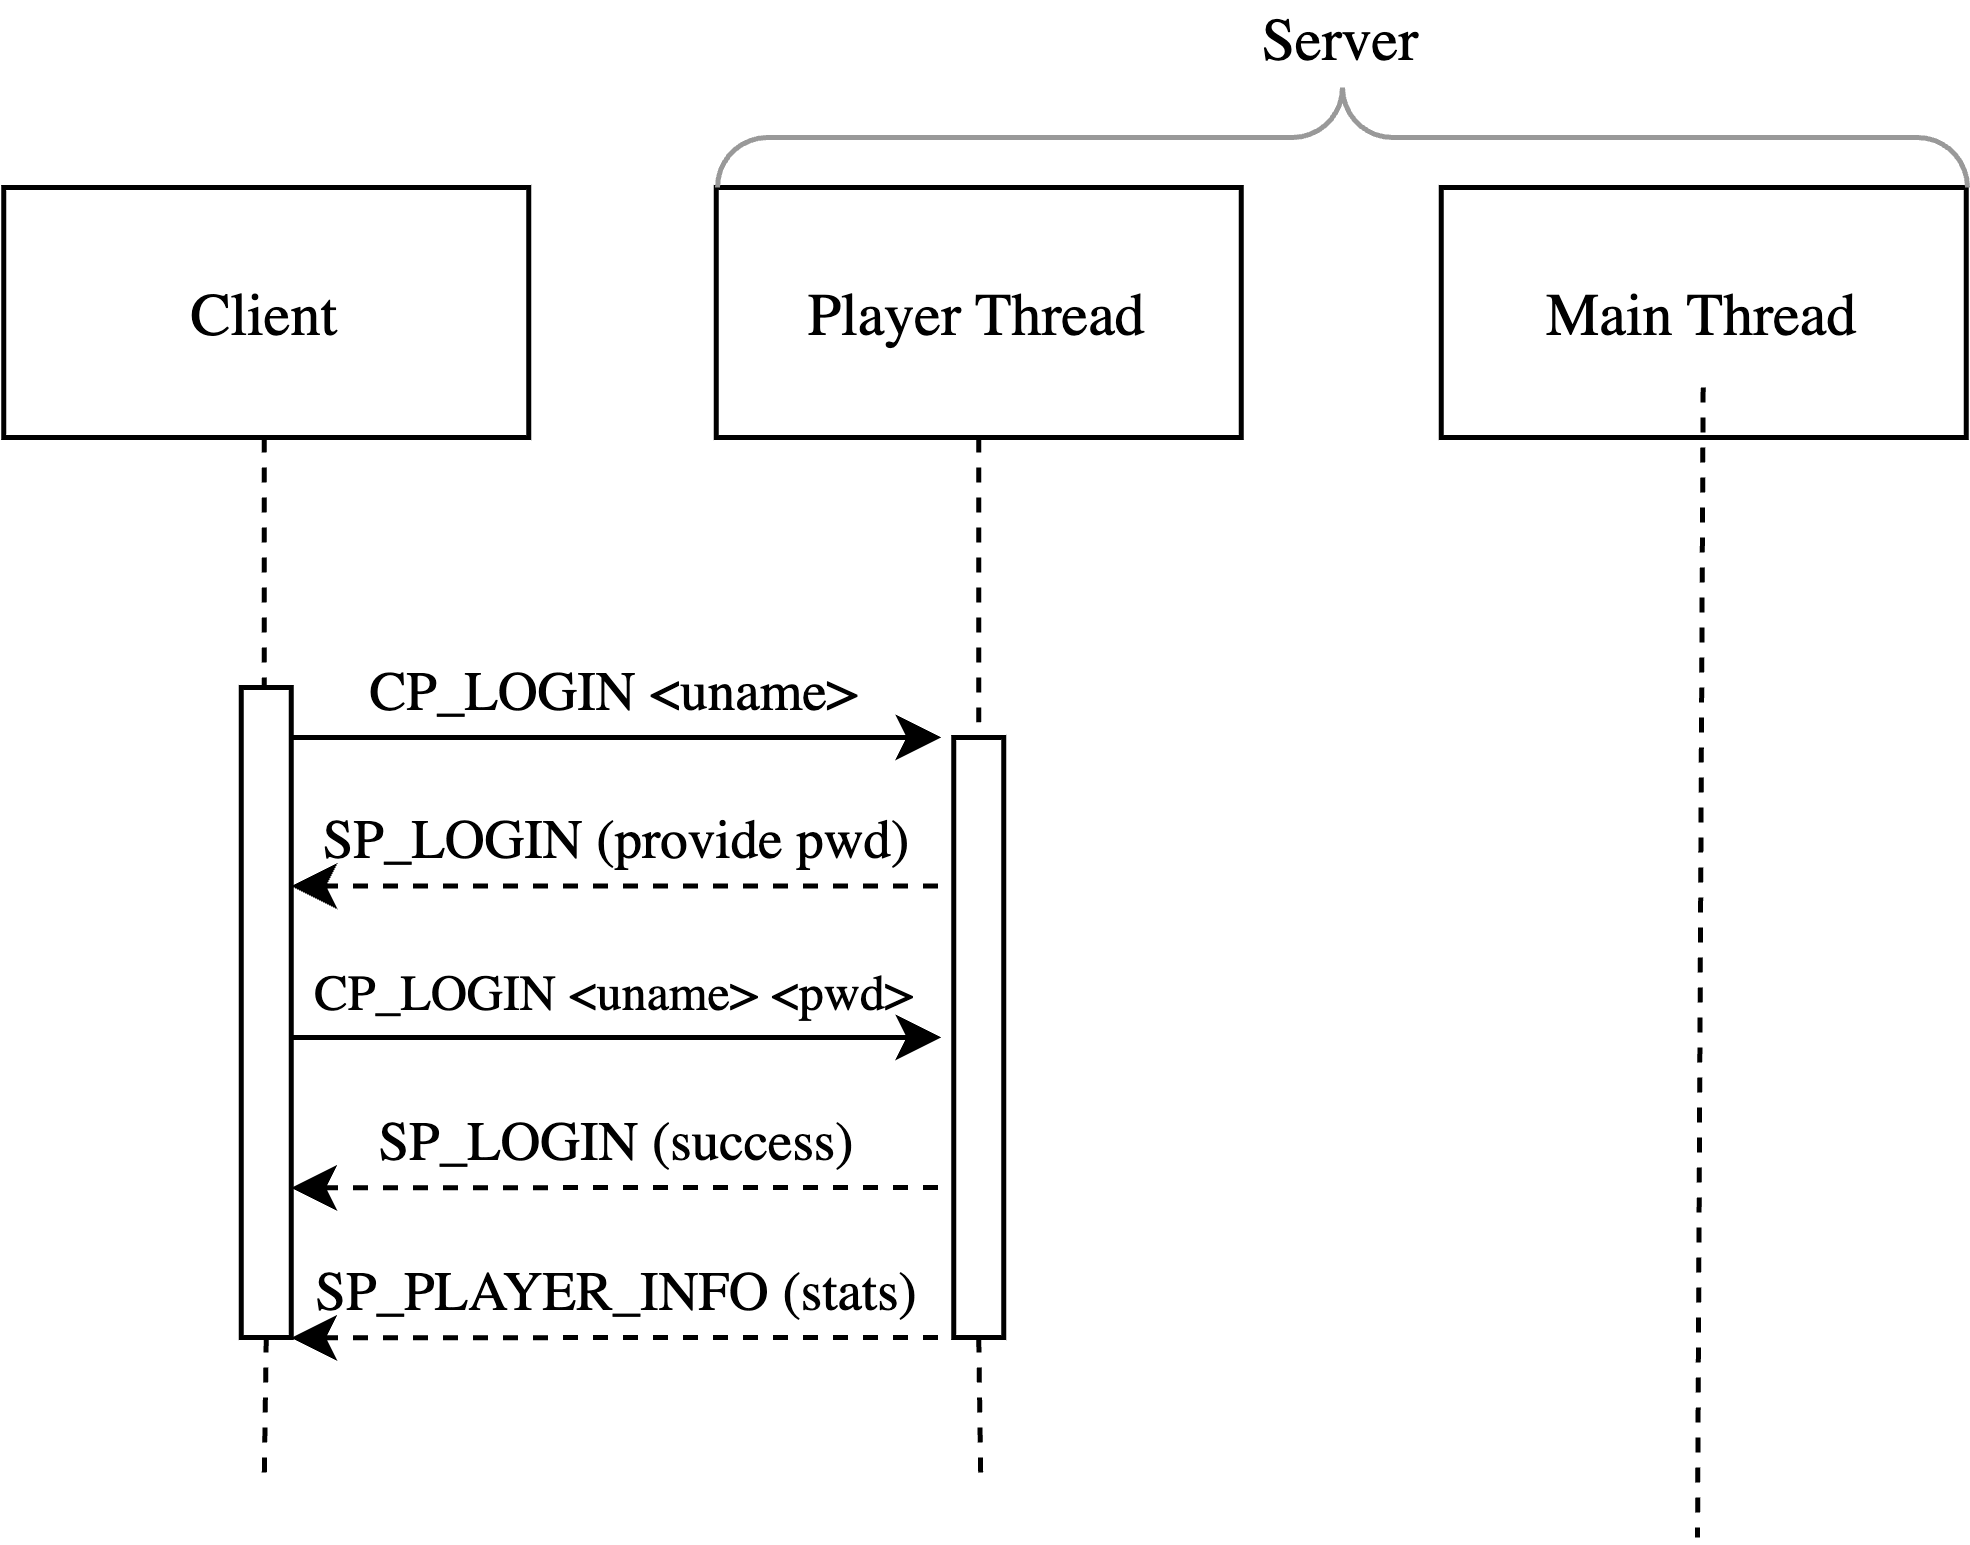
\includegraphics[width=\columnwidth]{figures/nt-login}
  \caption{A user logs in with a username for the first time on that server~\cite{netreksrc}.}
  \Description[]{}
\end{figure}
% Typical communication
\begin{figure}[h]
  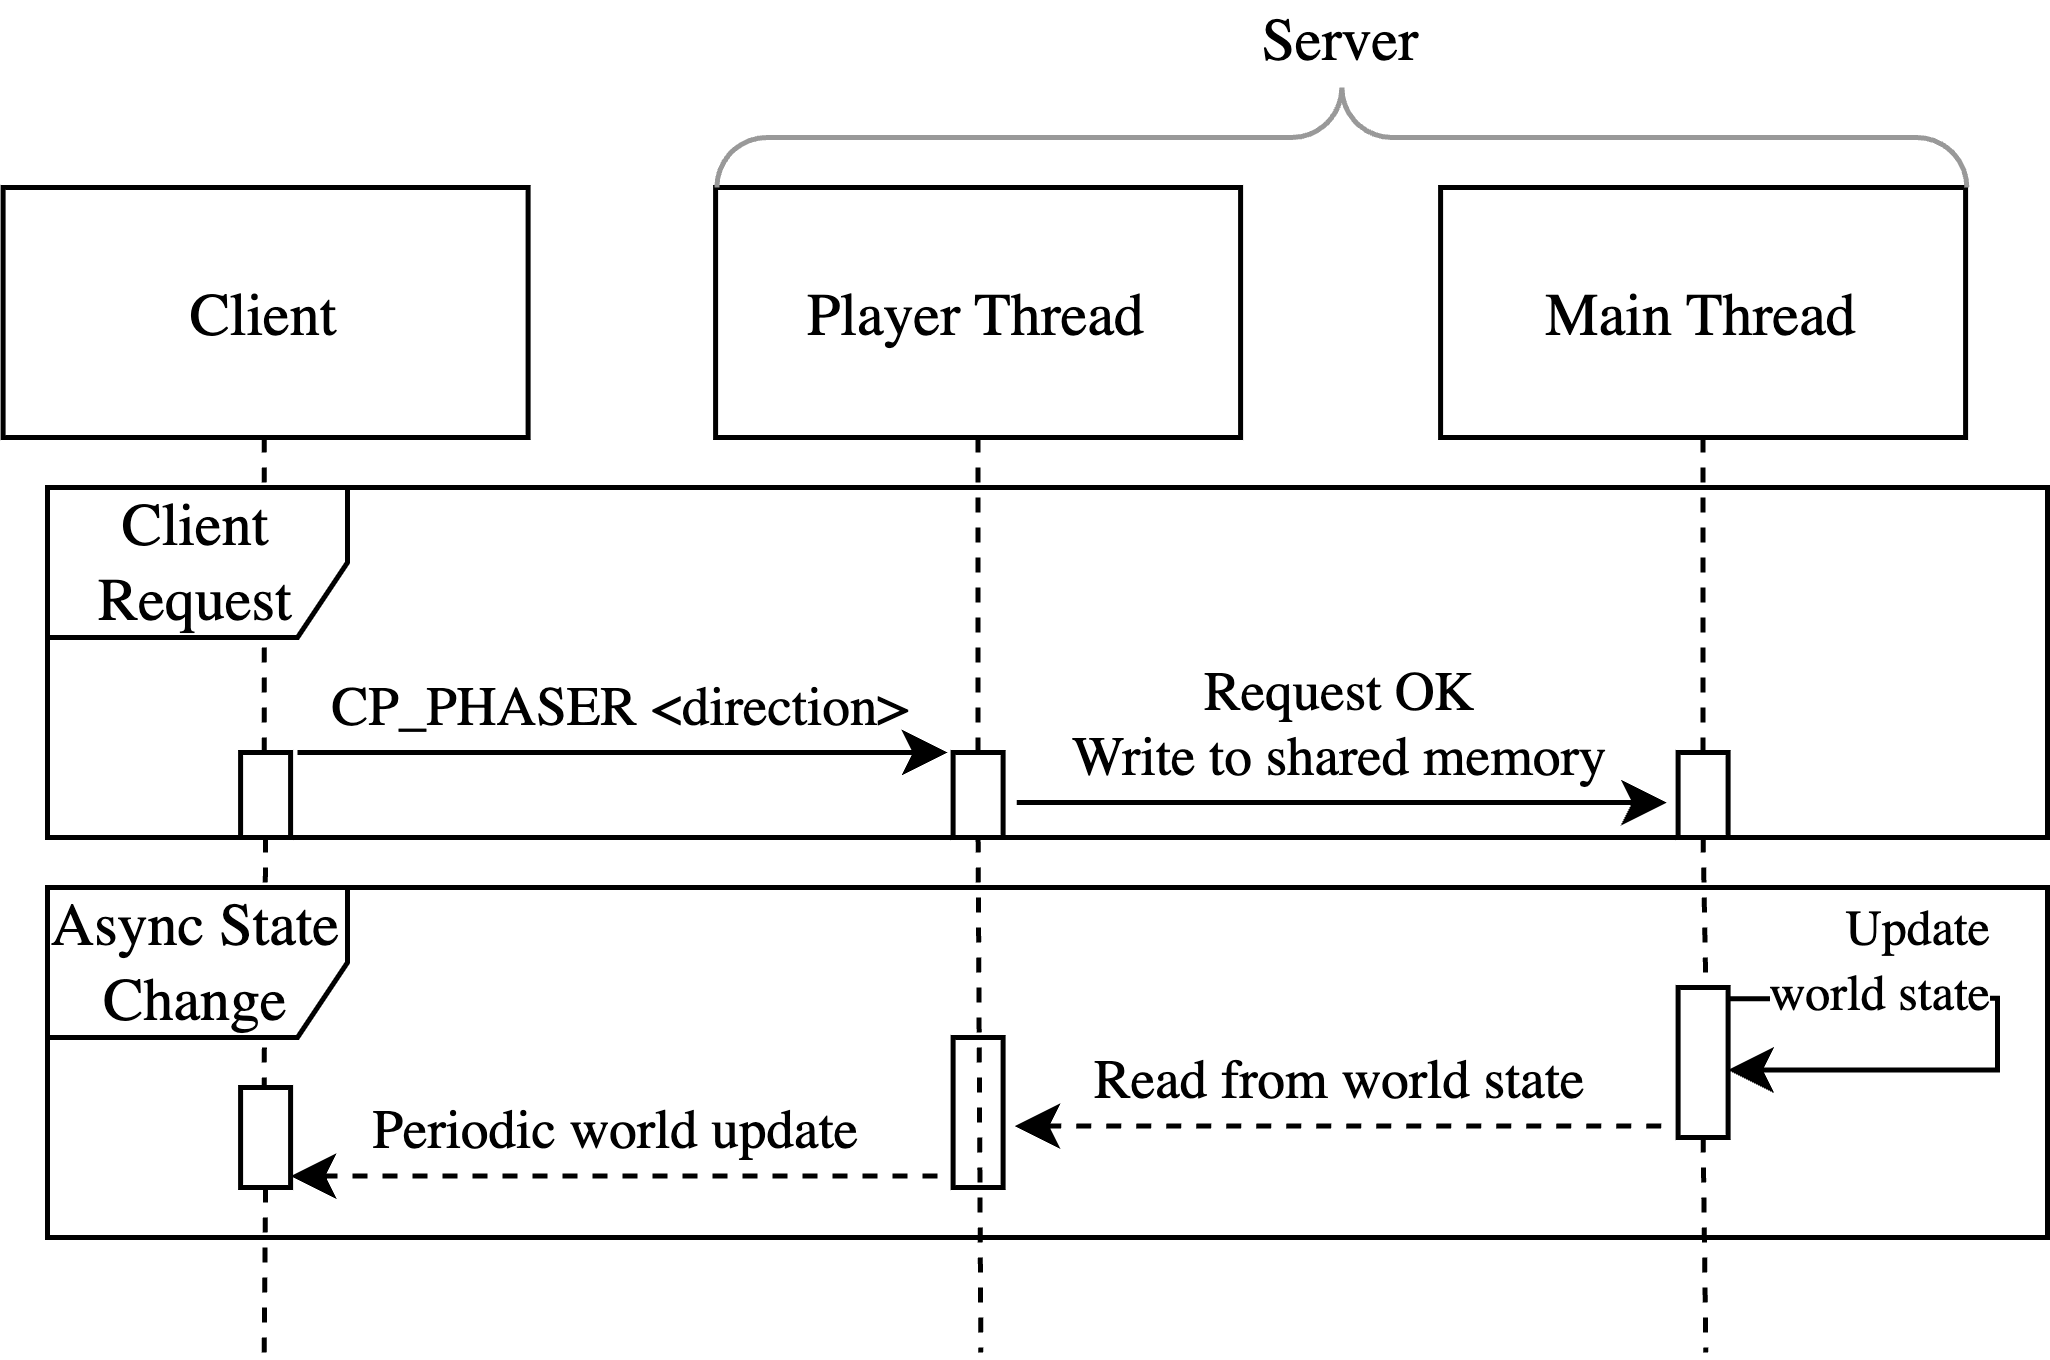
\includegraphics[width=\columnwidth]{figures/nt-typical}
  \caption{Typical gameplay flow. Note that the events in the lower frame can happen in any order~\cite{netreksrc}.}
  \Description[]{}
\end{figure}
% Reconnection
\begin{figure}[h!]
  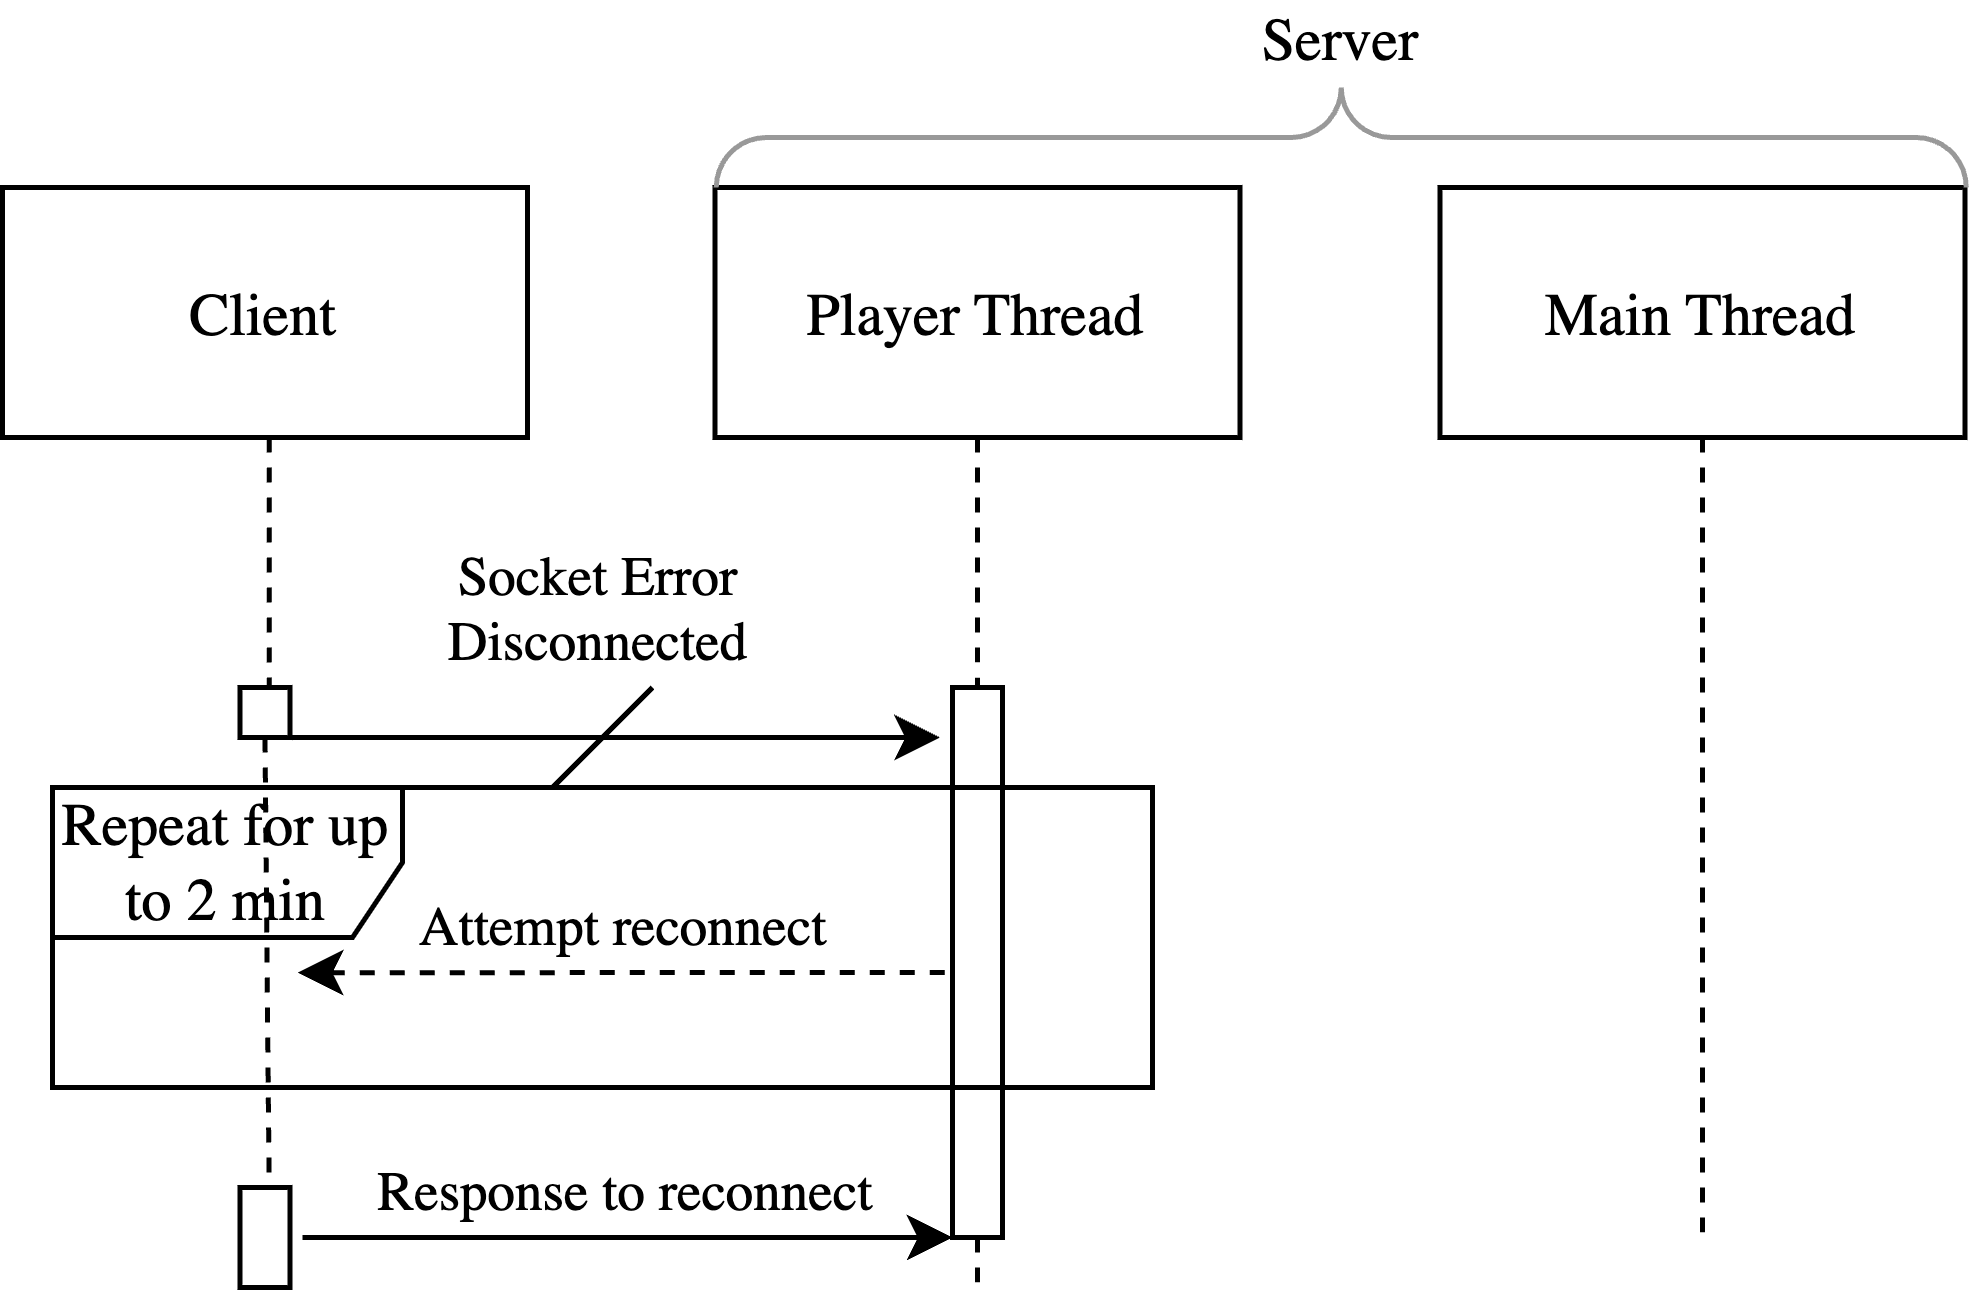
\includegraphics[width=\columnwidth]{figures/nt-recon}
  \caption{Reconnecting to a disconnected client~\cite{netreksrc}.}
  \Description[]{}
\end{figure}

\textit{Netrek}'s easy accessibility and high skill-ceiling gave it popularity in the mid-1990's and a loyal player base which still enjoys and develops the game today.
